\chapter{Model Development and Evaluation}
\section{Machine Learning Model}
Support vector machine and Multinomial NB model were trained in the training dataset given. Test dataset was used for the validation and generation of the classification report which is as follow. Multinomial NB was found to be perfoming better on test dataset with accuracy 0.58, f1-score 0.42 and weighted averate f1-score of 0.61.

\begin{figure}[H]
    \centering
    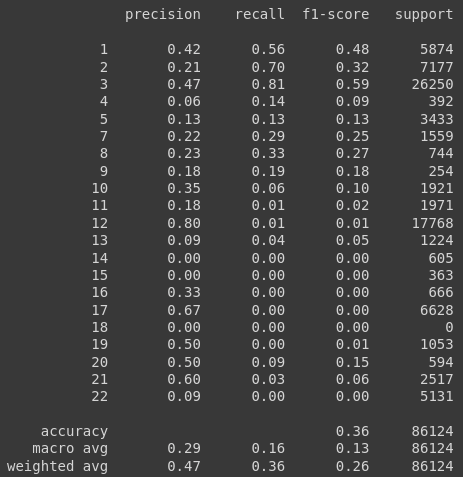
\includegraphics[scale = 0.7]{Model_cr_summary/svm_rc.png}
    \caption{SVM classification report}
    \label{fig:SVM classification report}
\end{figure}

\begin{figure}[H]
    \centering
    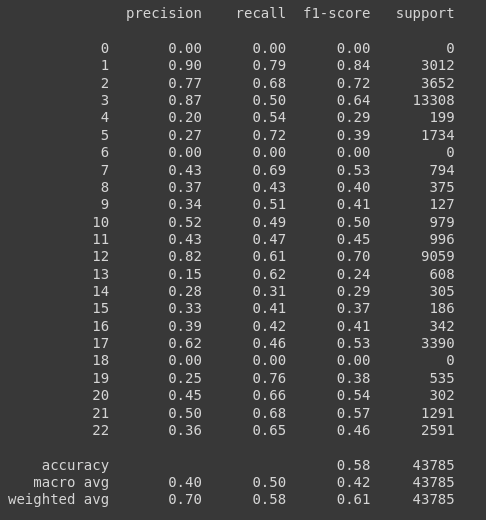
\includegraphics[scale = 0.7]{Model_cr_summary/multinomial_nb_cr.png}
    \caption{Multinomial NB classification report}
    \label{fig:Multinomial NB classification report}
\end{figure}


\section{LSTMs Dense Neural Network}
For training purpose, title and abstract of the training data were concatenated whose length distribution are shown below.

\begin{figure}[H]
    \centering
    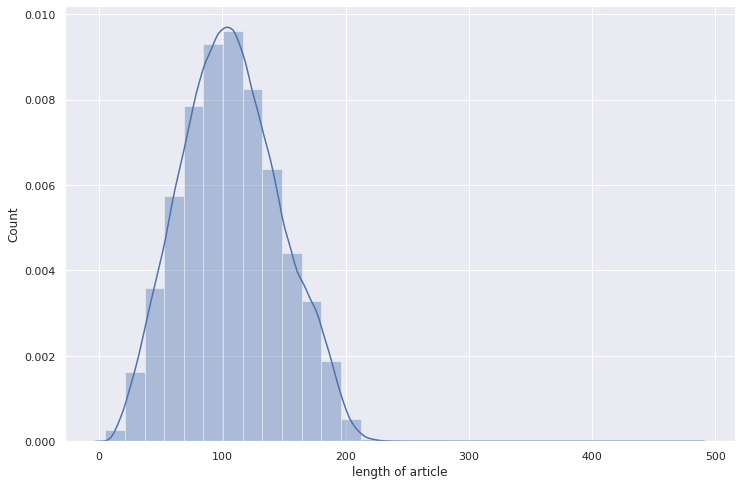
\includegraphics[scale = 0.6]{Model_cr_summary/text_length.png}
    \caption{Concatenated title and abstract length in training data}
    \label{fig:Concatenated title and abstract length in training data}
\end{figure}

From the above distribution of the text length for training data, we get the following statistics value:
\begin{table}[H]
    \begin{center}
        \begin{tabular}{ |c|c| }
            \hline
            mean               & 106.9657 \\
            \hline
            standard deviation & 39.87 \\
            \hline
            minimum            & 5       \\
            \hline
            first quartile     & 78      \\
            \hline
            median             & 105      \\
            \hline
            third quartile     & 134      \\
            \hline
            maximum            & 483     \\
            \hline
        \end{tabular}
    \end{center}
    \caption{Title and abstract length statistics based on word frequency}
    \label{table:Title and abstract length statistics based on word frequency}
\end{table}

Hence, we choose MAX\_PAD\_LENGTH = 140 for the tokenization of the data training the LSTMs Deep Neural Networks.

\subsection{Version 1}
Any label with count less than 5000 were over-sampled to 5000 and any label with count greater than 10,000 were under-sampled to 10,000 for training in this model. The model summary and the classification report are shown below.

\begin{figure}[H]
    \centering
    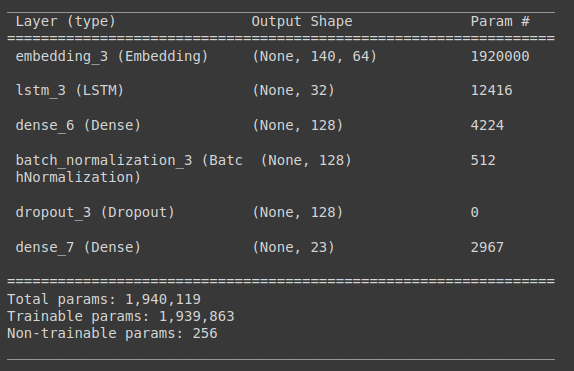
\includegraphics[scale = 0.7]{Model_cr_summary/sequential_v1_model.png}
    \caption{Model summary for version 1}
    \label{fig:Model summary for version 1}
\end{figure}

\begin{figure}[H]
    \centering
    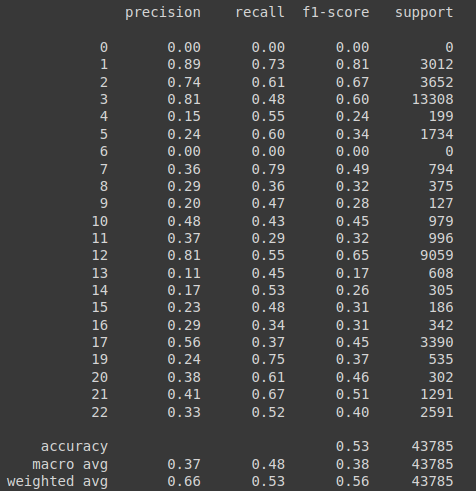
\includegraphics[scale = 0.7]{Model_cr_summary/sequential_v1_cr.png}
    \caption{Classification report for Version 1}
    \label{fig: Classification report for Version 1}
\end{figure}

\subsection{Version 2}
The model was same as in the Version 1. However, no. of LSTMs unit was reduced from 32 to 10 in this version and the result obtained were as follow. We can observe that the test accuracy improves from 0.53 to 0.68, macro average F1-score from 0.38 to 0.45.

\begin{figure}[H]
    \centering
    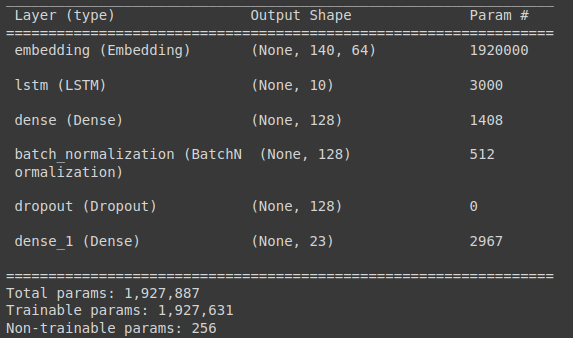
\includegraphics[scale = 0.7]{Model_cr_summary/sequential_v4_model.png}
    \caption{Model summary for version 2}
    \label{fig:Model summary for version 2}
\end{figure}

\begin{figure}[H]
    \centering
    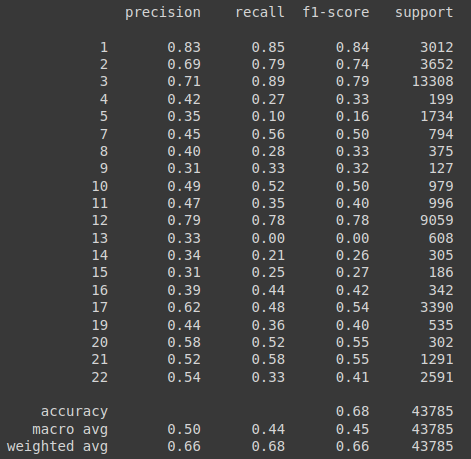
\includegraphics[scale = 0.6]{Model_cr_summary/sequential_v4_cr.png}
    \caption{Classification report for Version 2}
    \label{fig: Classification report for Version 2}
\end{figure}

The graph regarding loss, accuracy, f1-score and fbeta-score are as follow:

\begin{figure}[H]
    \centering
    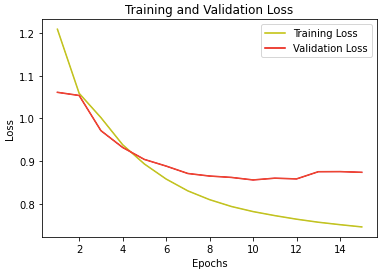
\includegraphics[scale = 0.6]{training_testing/seq_v4_loss.png}
    \caption{LSTMs V2 Loss curve}
    \label{fig:LSTMs V2 loss curve}
\end{figure}

\begin{figure}[H]
    \centering
    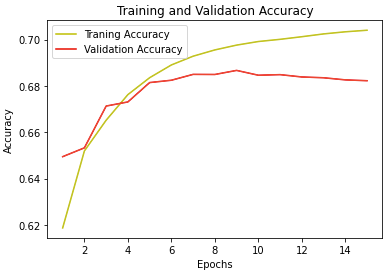
\includegraphics[scale = 0.6]{training_testing/seq_v4_accuracy.png}
    \caption{LSTMs V2 accuracy curve}
    \label{fig:LSTMs V2 accuracy curve}
\end{figure}

\begin{figure}[H]
    \centering
    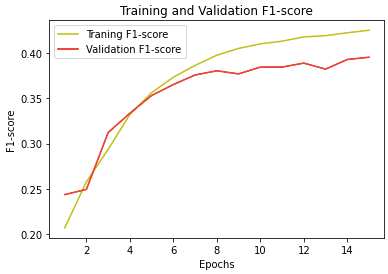
\includegraphics[scale = 0.6]{training_testing/seq_v4_f1.png}
    \caption{LSTMs V2 F1-score curve}
    \label{fig:LSTMs V2 F1-score curve}
\end{figure}

\begin{figure}[H]
    \centering
    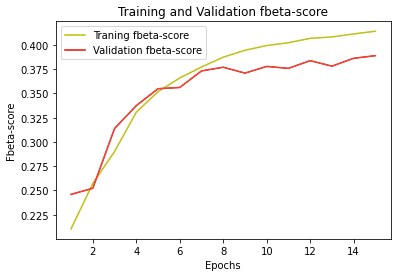
\includegraphics[scale = 0.6]{training_testing/seq_v4_beta.png}
    \caption{LSTMs V2 fbeta-score curve}
    \label{fig:LSTMs V2 fbeta-score curve}
\end{figure}

\section{Transformer Model}
We can observe form the classification report that the accuracy improves to 0.69 and macro average f1-score to 0.46.

\begin{figure}[H]
    \centering
    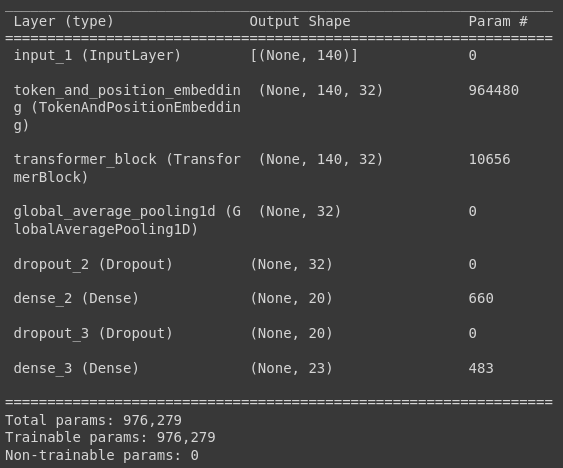
\includegraphics[scale = 0.55]{Model_cr_summary/transformer_v1_model.png}
    \caption{Transformer Model summary for version 1}
    \label{fig:Transformer Model summary for version 1}
\end{figure}

\begin{figure}[H]
    \centering
    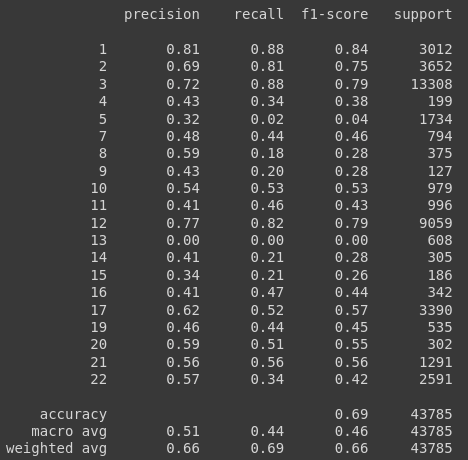
\includegraphics[scale = 0.6]{Model_cr_summary/transformer_v1_cr.png}
    \caption{Transformer Classification report for Version 1}
    \label{fig:Transformer Classification report for Version 1}
\end{figure}

The graph regarding loss, accuracy, f1-score and fbeta-score are as follow:

\begin{figure}[H]
    \centering
    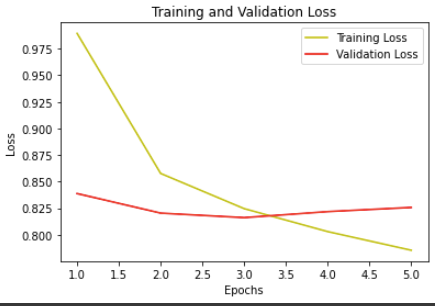
\includegraphics[scale = 0.6]{training_testing/transformer_v1_loss.png}
    \caption{Transformer V1 Loss curve}
    \label{fig:Transformer V1 loss curve}
\end{figure}

\begin{figure}[H]
    \centering
    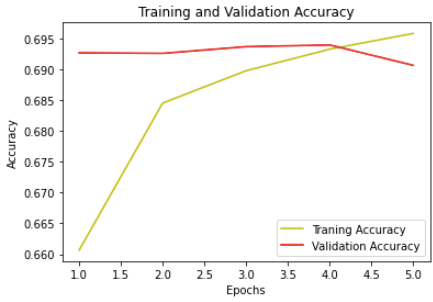
\includegraphics[scale = 0.6]{training_testing/transformer_v1_accuracy.png}
    \caption{Transformer V1 accuracy curve}
    \label{fig:Transformer V1 accuracy curve}
\end{figure}

\begin{figure}[H]
    \centering
    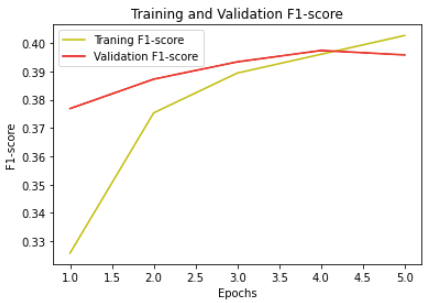
\includegraphics[scale = 0.6]{training_testing/transformer_v1_f1.png}
    \caption{Transformer F1-score curve}
    \label{fig:Transformer F1-score curve}
\end{figure}

\begin{figure}[H]
    \centering
    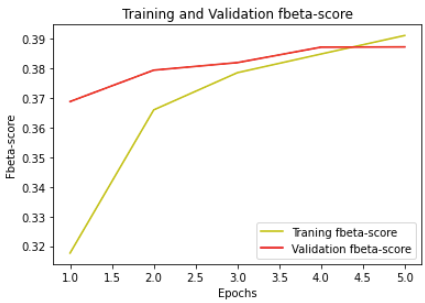
\includegraphics[scale = 0.6]{training_testing/transformer_v1_beta.png}
    \caption{Transformer V1 fbeta-score curve}
    \label{fig:Transformer V1 fbeta-score curve}
\end{figure}

